\documentclass{article}
\usepackage{fancyhdr}
\usepackage{ctex}
\usepackage{listings}
\usepackage{graphicx}
\usepackage[a4paper, body={18cm,22cm}]{geometry}
\usepackage{amsmath,amssymb,amstext,wasysym,enumerate,graphicx}
\usepackage{float,abstract,booktabs,indentfirst,amsmath}
\usepackage{array}
\usepackage{booktabs}
\usepackage{multirow}
\usepackage{url}
\usepackage{diagbox}
\renewcommand\arraystretch{1.4}
\usepackage{indentfirst}
\setlength{\parindent}{2em}
\usepackage{enumitem}
\setmonofont{Consolas}
\usepackage{listings}
\usepackage{xcolor}
\usepackage{makecell}
\usepackage{tikz}
\usetikzlibrary{positioning, arrows.meta}
\setCJKmonofont{黑体}
\lstset{  
	% 基本设置  
	xleftmargin = 3em, xrightmargin = 3em, aboveskip = 1em,  
	backgroundcolor = \color{white},  
	basicstyle = \small\ttfamily,  
	rulesepcolor = \color{gray},  
	breaklines = true,  
	numbers = left,  
	numberstyle = \small,  
	numbersep = -14pt,  
	frame = shadowbox,  
	showspaces = false,  
	columns = fixed,  
	sensitive = true,  
	% VSCode 风格配色  
	keywordstyle = \color{blue!70!black}\bfseries,  
	emphstyle = \color{red!70!black}\bfseries, % 对于强调的词  
	emphstyle=[2]\color{purple!70!black}\bfseries, % 对于第二组强调的词  
	commentstyle = \color{green!60!black}, % 注释颜色  
	stringstyle = \color{orange!90!black}, % 字符串颜色更亮一些  
	morekeywords={ASSERT, int64\_t, uint32\_t},  
	moreemph={ASSERT, NULL},  
	moreemph=[2]{int64\_t, uint32\_t, tid\_t, uint8\_t, int16\_t, uint16\_t, int32\_t, size\_t, bool},  
	morecomment=[l][\color{green!60!black}]{+}, % 以+开头的注释  
}

%--------------------页眉--------------------%
\pagestyle{fancy}
\fancyhead[L]{华东师范大学}
\fancyhead[R]{East China Normal University}
\fancyhead[C]{}
\fancyfoot[C]{-\thepage-}
\renewcommand{\headrulewidth}{1.5pt}
%--------------------标题--------------------%
\begin{document}
\begin{center}
  {\Large{\textbf{\heiti 实验一:基于正向最大匹配算法的分词}}}
  \begin{table}[H]
    \centering
    \begin{tabular}{p{2cm}p{4cm}<{\centering}p{1cm}p{2cm}p{6cm}<{\centering}}
      课程名称:    & 自然语言处理 & \quad & 指导教师:    & 张蓉
      \\ \cline{2-2} \cline{5-5}
      姓\qquad 名: & 王海生    & \quad & 学\qquad 号: & 10235101559
      \\ \cline{2-2} \cline{5-5}
    \end{tabular}
  \end{table}
  \textbf{代码仓库:}\url{https://github.com/Hanson-Wang-chn/ECNU-NLP-WHS.git}
\end{center}
\rule{\textwidth}{1pt}
%--------------------正文--------------------%
\section{实验结果}

\begin{figure}[H]
	\centering
	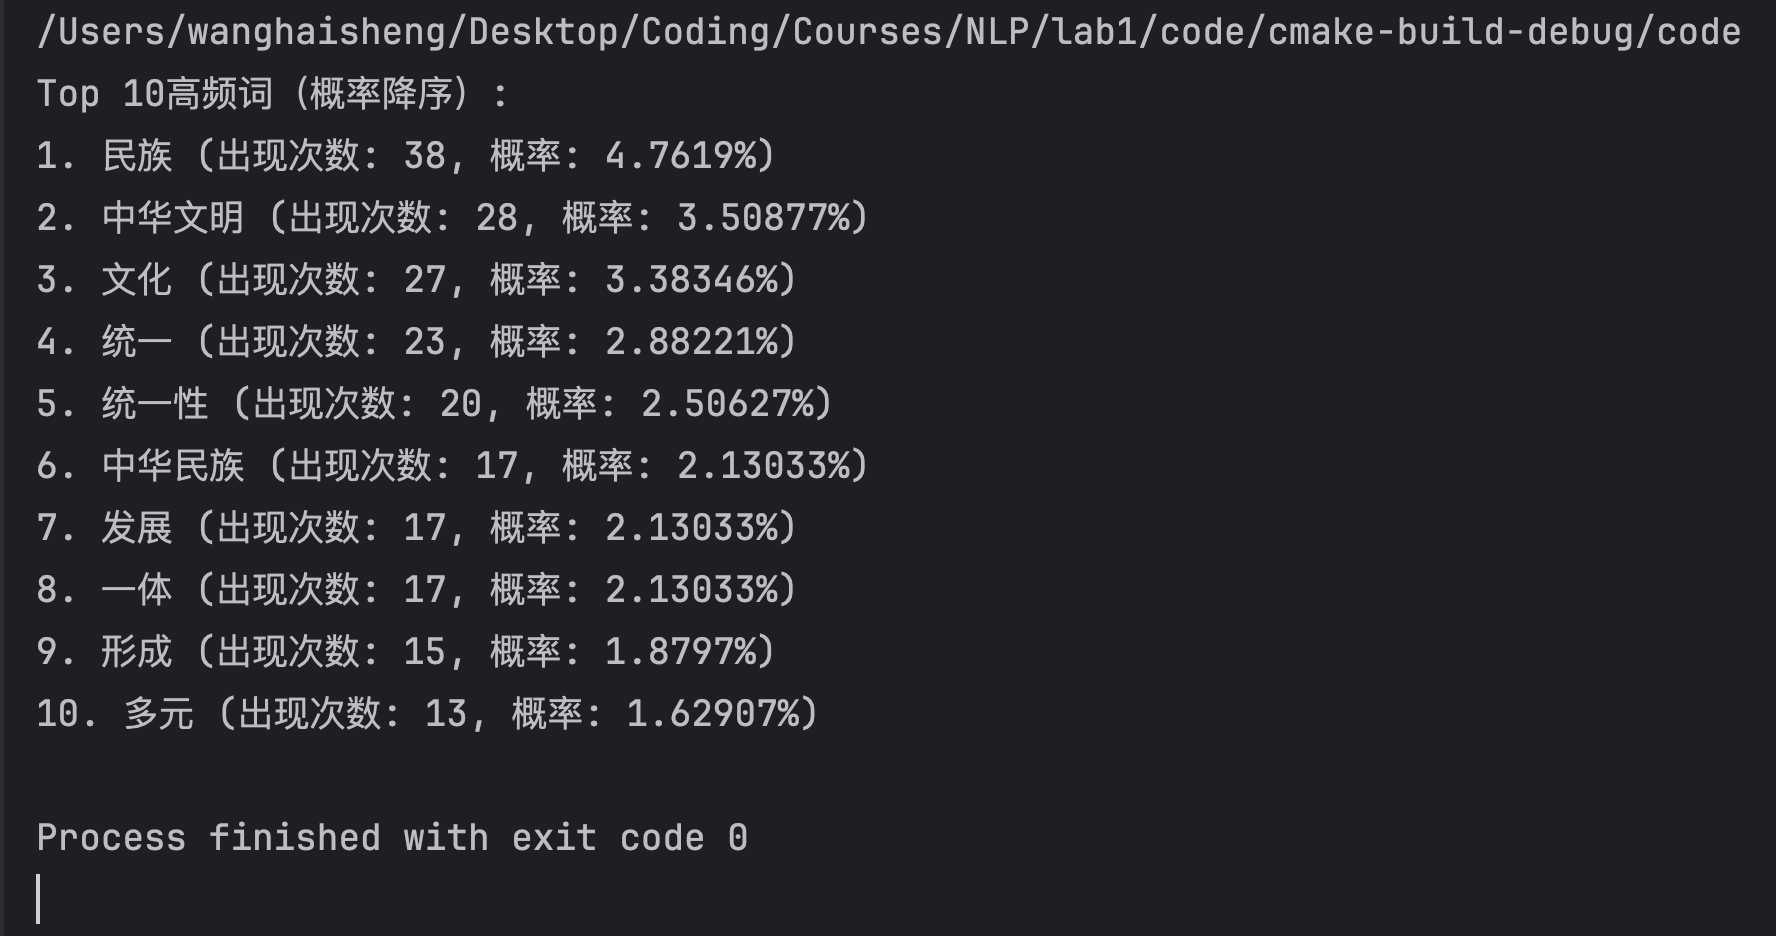
\includegraphics[width=0.7\textwidth]{img/result.png}
	\caption{实验结果}
\end{figure}

\section{正向匹配算法}

最大正向匹配分词算法(Forward Maximum Matching, FMM)是一种基于\textbf{词典}的自然语言处理方法,核心思想是从文本的\textbf{开头}开始逐步向前推进,尝试寻找\textbf{最长}且位于预定义词汇表中的词组来进行切割。

\subsection{算法步骤}

\begin{figure}[H]
	\centering
	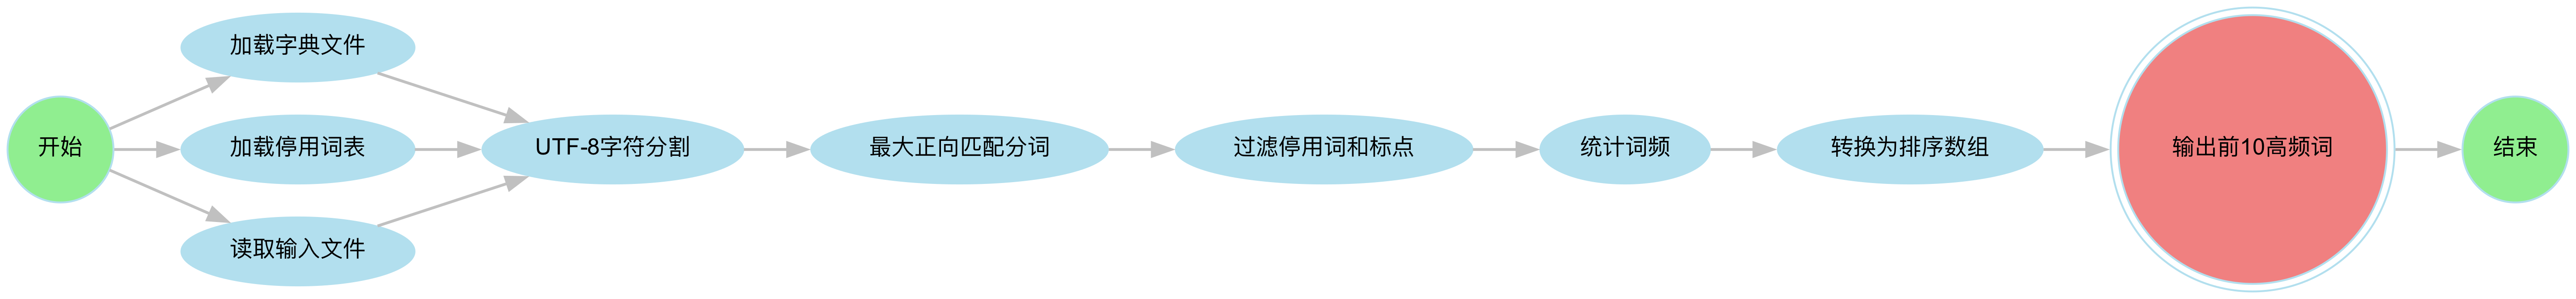
\includegraphics[width=1.0\textwidth]{img/algorithm_flowchart.png}
	\caption{最大正向匹配分词算法示意图}
\end{figure}

\begin{enumerate}
	\item 加载字典文件、停用词表: 读取词典文件、停用词表,分别放入一个无需集合(代码中使用哈希表实现)中。
	\item 读取输入文件: 读取待分析的\texttt{.txt}文件。
	\item \texttt{UTF-8}字符分割: 由于需要处理中文汉字,有必要把所有的字符统一为\texttt{UTF-8}编码。在实践中,忽略这一步会导致乱码。
	\item 最大正向匹配分词: 内外两个循环。内循环从最大长度开始递减,直至匹配;外循环遍历待处理文本。
	\item 过滤停用词和标点: 移除分词结果中的停用词及标点符号。
	\item 统计词频: 计算每种词汇在文本中出现的次数,并记录总数。
	\item 转换为排序数组: 将统计得到的词频数据转换成一个数组,并按照出现频率从高到低进行排序。
	\item 输出高频词: 显示出现频率最高的前10个词汇及其对应的出现概率。
\end{enumerate}

\subsection{算法分析}

\begin{enumerate}
	\item \textbf{优点:}实现简单;非常适合\textbf{处理长词}。
	\item \textbf{缺点:}难以处理词典中不存在的词(每个汉字均作为一个词),性能依赖于词典,灵活性较差。
	\item \textbf{其他算法:}
	
	\begin{itemize}
		\item \textbf{最大逆向匹配:}实现复杂度稍高,能更好地处理某些歧义情况。
		\item \textbf{双向最大匹配:}计算量稍大,结合正向匹配和逆向匹配的优点。
		\item \textbf{基于统计或深度学习的算法:}不再依赖于词典,效果较好,但需要较大的算力和数据集。
	\end{itemize}
\end{enumerate}

\section{\texttt{C++}代码创新点}

由于本次实验的代码使用\texttt{C++}编写,没有\texttt{Python}中的一些分词库,所以必须从头开始设计算法和数据结构。我认为,我的代码中的亮点是,使用了\textbf{哈希表}作为保存词表的数据结构,大幅降低了算法的时间复杂度。

具体来说,我使用\texttt{unordered\_set}作为存储字典文件和停用词表的无序集合,使用\texttt{unordered\_map}来一一对应词和该词的频率。

\begin{lstlisting}[language=C++]
	unordered_set<string> loadDictionary(const string& path); // 字典
	unordered_set<string> loadStopwords(const string& path); // 停用词表
	unordered_map<string, int> freq; // 词和频率
\end{lstlisting}

借这次实验的机会,除最大正向匹配分词算法之外,我还熟悉了\texttt{C++ STL}的原理和使用。这算是比较大的收获。

\end{document}